\documentclass[11pt]{article}

% ----------------------------------------------------------------------------
%  Development of the Monash True-Triaxial Hopkinson Bar System and an
%  Integrated Digital Twin for Multiaxial Dynamic Rock Characterisation
%
%  Draft generated to demonstrate the advancement of the Monash Tri-HB system.
%  Figures are produced by the Virtual Tri-HB Streamlit workspace
%  (scripts/export_handbook_step_figures.py, export_handbook_mode_figures.py,
%   export_paper_schematic.py).
% ----------------------------------------------------------------------------

\usepackage[a4paper,margin=2.4cm]{geometry}
\usepackage{lmodern}
\usepackage[T1]{fontenc}
\usepackage[utf8]{inputenc}
\usepackage{amsmath,amssymb}
\usepackage{graphicx}
\usepackage{subcaption}
\usepackage{booktabs}
\usepackage{siunitx}
% siunitx v3 removed \SI and \SIrange; provide them if absent (matches Handbook).
\providecommand{\SI}[2]{\qty{#1}{#2}}
\providecommand{\SIrange}[3]{\qtyrange{#1}{#2}{#3}}
\providecommand{\diameter}{\ensuremath{\varnothing}}
\usepackage{microtype}
\usepackage{xcolor}
\usepackage{authblk}
\usepackage[hidelinks]{hyperref}
% RMRE / Springer use author--year citations. biblatex (authoryear) + biber is
% used here because the Springer svjour3/sn-jnl class files are not available in
% this TeX installation; the structure (title block, declarations, author--year
% references) follows the Rock Mechanics and Rock Engineering conventions.
\usepackage[style=authoryear,natbib=true,backend=biber,maxcitenames=2,%
            maxbibnames=99,giveninits=true,uniquename=false,doi=true,url=false,isbn=false]{biblatex}
\addbibresource{refs.bib}
\renewcommand*{\bibfont}{\small}

\graphicspath{{figures/}{../Handbook/figures/handbook_steps/}{../Handbook/figures/handbook_modes/}}

\sisetup{detect-all}
\renewcommand{\arraystretch}{1.15}
\setlength{\parskip}{2pt}

\newcommand{\Cz}{C_{0}}
\newcommand{\eps}{\varepsilon}
\newcommand{\epsd}{\dot{\varepsilon}}

\title{\bfseries Development of the Monash True-Triaxial Hopkinson Bar System
and an Integrated Digital Twin for Multiaxial Dynamic Rock Characterisation}

\author[1]{Q.~B.~Zhang\thanks{Corresponding author: \texttt{qianbing.zhang@monash.edu}}}
\affil[1]{Department of Civil and Environmental Engineering, Monash University, Clayton, VIC 3800, Australia}

\date{\normalsize Prepared for submission to \textit{Rock Mechanics and Rock Engineering}\\[2pt]\small\today}

\begin{document}
\maketitle

\begin{abstract}
\noindent
Conventional split-Hopkinson pressure bar (SHPB) testing characterises rock
under one-dimensional dynamic loading, yet rock in deep mining, tunnelling and
rock blasting fails under \emph{multiaxial} stress states at high strain rate.
This paper presents the development of the Monash triaxial Hopkinson bar
(Tri-HB) --- a gas-gun-driven system of three independent pairs of orthogonal
square bars with hydraulic confinement on all three axes, enabling true-triaxial
($\sigma_2\neq\sigma_3$) static--dynamic coupled loading --- and an integrated
\emph{digital twin}, the Virtual Tri-HB, that unifies test design, three-wave
data reduction, stress-path interpretation and damage modelling in a single
six-step workflow. We report four advances embedded in the digital twin: (i) a
unified treatment of four loading families and six physics modes spanning
uniaxial SHPB to electromagnetic programmable multiaxial loading; (ii) a
true-triaxial, Lode-angle-dependent and rate-dependent failure envelope that
captures the intermediate principal stress effect with the correct sign; (iii) a
thermodynamically consistent damage-energy partition in which the first law
closes by construction, $W_{\mathrm{input}}=W_{\mathrm{el}}+W_{\mathrm{diss}}$;
and (iv) an orthotropic damage tensor whose components are driven by the
directional tensile strain, reproducing the directional (axial-splitting)
fracture of rock blasting. Because the three orthogonal bars measure
direction-resolved stress, strain and wave speed, each component of the damage
tensor can in principle be calibrated independently --- a capability a uniaxial
SHPB cannot provide. We close with a calibrate-then-blind-predict validation
roadmap that positions the Tri-HB and its digital twin for quantitative,
multiaxial dynamic constitutive modelling of rock.
\end{abstract}

\noindent\textbf{Keywords:} triaxial Hopkinson bar; dynamic rock mechanics;
true-triaxial loading; intermediate principal stress; anisotropic damage; rock
blasting; digital twin.

\section{Introduction}\label{sec:intro}

The dynamic mechanical response of rock governs the safety and efficiency of
deep underground excavation, rockburst mitigation and rock blasting, where
loading rates of $10^{1}$--$10^{3}\,\mathrm{s}^{-1}$ coincide with confining
stresses of tens to hundreds of megapascals~\citep{zhang2014,xia2015}. Capturing
this response in the laboratory has driven more than a century of development of
the Hopkinson bar, yet the classical apparatus remains one-dimensional. This
section traces that development, examines how confinement has conventionally been
added, and motivates a true-triaxial alternative.

\subsection{From the Hopkinson bar to the split-Hopkinson pressure bar}

The technique originates with Bertram Hopkinson, who in 1914 used a long elastic
bar terminated by a momentum trap to record the pressure--time history produced
by explosive detonation and bullet impact~\citep{hopkinson1914} --- the original
\emph{Hopkinson pressure bar}. \citet{davies1948} replaced the mechanical
momentum measurement with electrical (condenser) sensing of bar displacement and
gave the first rigorous treatment of geometric wave dispersion.
\citet{kolsky1949} then split the bar in two and placed a thin specimen between
an incident and a transmission bar: the incident, reflected and transmitted
pulses recovered from bar gauges yield the specimen stress, strain rate and
strain, defining the split-Hopkinson pressure bar (SHPB), or Kolsky bar, still in
use today. Subsequent maturation added resistance strain-gauge instrumentation,
Pochhammer--Chree dispersion correction, and pulse shaping to enforce a constant
strain rate and stress equilibrium in brittle specimens~\citep{frew2002}; the
method was extended to tension, torsion and elevated temperature, and codified
for rock through suggested methods and reviews~\citep{zhou2012,zhang2014,xia2015}.
Throughout, however, the loading remained \emph{one-dimensional}: a single axial
pulse on an unconfined specimen.

\subsection{Confined and triaxial-chamber dynamic testing}

Because rock in situ is confined, dynamic testing under lateral pressure followed
soon after. Two strategies became standard. In \emph{passive} confinement a rigid
metal sleeve or shrink-fit ring surrounds the specimen and supplies a reactive
radial constraint that rises with the axial load but is not independently
controlled~\citep{christensen1972}. In \emph{active} confinement the SHPB specimen
is enclosed in a pressure cell and a hydraulic or pneumatic medium imposes a
prescribed confining pressure before the dynamic axial pulse
arrives~\citep{lindholm1974}. These confined-SHPB methods established the pressure
dependence and dynamic increase of rock strength and remain widely used; they
correspond to the confinement-chamber mode (Mode~2) of the present workflow. They
share, however, three intrinsic limitations. First, the confinement is
\emph{axisymmetric}, $\sigma_2=\sigma_3$, so the \emph{intermediate principal
stress effect} --- shown by quasi-static true-triaxial testing to be first-order
for rock strength~\citep{mogi1971} --- cannot be accessed. Second, the confinement
is quasi-static and pre-applied; the lateral stress can be neither pulsed nor
timed relative to the axial event. Third, the specimen is enclosed, so the
lateral stress and strain are inferred through the cell rather than measured
directly, and the lateral dynamic (Poisson-driven) response is not resolved.

From a boundary-value standpoint, the confining medium acts as a low-impedance
\emph{traction} boundary rather than a displacement constraint. On the wetted
specimen surface $S$ with outward normal $\mathbf{n}$, an inviscid fluid transmits
only a normal pressure and couples to the wall acceleration through
\begin{equation}
\sigma_{ij}n_j=-p(t)\,n_i,\qquad
\frac{\partial p}{\partial n}=-\rho_f\,\ddot{u}_n,
\label{eq:fluidbc}
\end{equation}
the first a Neumann (traction) condition that leaves the lateral displacement
free, the second the fluid--structure coupling that fixes any radiated energy.
The acoustic mismatch with the rock, $R_{\mathrm{lat}}=(Z_f-Z_s)/(Z_f+Z_s)$ with
$Z=\rho c$, is severe --- $Z_f/Z_s\sim10^{-1}$ for liquids and $\lesssim10^{-3}$
for gases --- so the surface behaves almost as a pressure-release boundary and
radiates little, while the chamber pressure stays effectively quasi-static,
$p\approx p_c$, over the $\sim\!100\,\mu\mathrm{s}$ event. The confinement is thus
a clean axisymmetric pressure ($\sigma_2=\sigma_3=p_c$) that neither suppresses
lateral expansion nor yields a measurable lateral signal.

These chamber effects can be mitigated, and the relations above prescribe how.
The dynamic pressure rise, $\Delta p\approx K_{\mathrm{eff}}(V_s/V_f)\,2\nu\varepsilon_{\mathrm{ax}}$,
is held well below $p_c$ by a large reservoir ($V_f\gg V_s$) or a soft medium ---
a gas, with $K_{\mathrm{eff}}=\gamma p_c$, is about two orders of magnitude better
than hydraulic oil. Radiation into the medium is suppressed by smooth, long-wavelength
loading ($ka\ll1$, the same condition that controls bar dispersion); wall
reflections are excluded from the measurement window $t_w$ by sizing the chamber
radius $d>c_f t_w/2$; and parasitic load paths are removed with a thin, soft
sealing jacket ($A_jE_j\ll A_sE_s$) and non-load-bearing seals. Each remedy,
however, only \emph{mitigates} a low-impedance, enclosed boundary, and none
recovers the lateral signal --- the gap the next section closes by replacing the
chamber with matched-impedance bars.

\subsection{The case for a true-triaxial Hopkinson bar}

The Monash triaxial Hopkinson bar (Tri-HB) removes the confining chamber
altogether and instead loads a cubic specimen through \emph{three independent
pairs of orthogonal Hopkinson bars}, with hydraulic cylinders applying
independent quasi-static pre-stress on each axis and a gas gun superposing the
dynamic pulse on the $X$ axis. Each limitation above becomes a capability.
(i)~\emph{True-triaxial} states, $\sigma_1>\sigma_2>\sigma_3$, are imposed by
setting the three pre-stresses independently, so the intermediate-stress and
Lode-angle dependence can be probed dynamically. (ii)~\emph{Static--dynamic
coupling} reproduces the in-situ condition of a pre-stressed rock mass struck by a
dynamic disturbance, as in blasting or rockburst. (iii)~The lateral response is
\emph{measured directly}: each transverse axis carries its own output bars and
gauges (six gauge sets in total), so $\sigma_y$, $\sigma_z$ and the directional
fracture are resolved rather than inferred. (iv)~With programmable electromagnetic
topologies the per-axis pulses can be timed independently, enabling loading-path
and sequence studies a chamber cannot provide.

These hardware capabilities become quantitative only if the interpretation keeps
pace. Reducing a multiaxial dynamic test to a constitutive statement requires a
consistent three-wave analysis on each axis, a failure surface that depends on all
three stress invariants, a thermodynamically admissible energy balance, and a
damage description that is \emph{directional} --- because blasting produces
oriented cracks rather than isotropic softening. These ingredients are rarely
assembled in one auditable workflow.

\subsection{Scope and outline}

This paper presents the Tri-HB system together with an integrated digital twin
that couples the hardware data-reduction equations to such a constitutive
framework. Section~\ref{sec:system} describes the hardware and its four loading
families; Section~\ref{sec:reduction} the one-dimensional wave propagation, the
per-axis three-wave reduction, and the wave-interaction regime map; and
Section~\ref{sec:twin} the integrated digital twin. Section~\ref{sec:advances} presents the three constitutive advances --- the
true-triaxial rate-dependent envelope, the energy-consistent dissipation, and the
orthotropic damage tensor. Section~\ref{sec:roadmap} gives the validation roadmap,
and Section~\ref{sec:conclusion} concludes. All figures are generated by the
Virtual Tri-HB workspace from prescribed-pulse reference cases; the present
contribution is the system and its modelling framework, with experimental
calibration identified as the immediate next step.

\section{The Monash Tri-HB system}\label{sec:system}

\subsection{Hardware configuration}

The Tri-HB (Fig.~\ref{fig:schematic}) couples a gas-gun dynamic loading train on
the $X$ axis with three independent pairs of orthogonal square bars and hydraulic
confinement on all three axes. The dynamic train comprises a cylindrical striker
($\diameter\SI{40}{mm}$, length \SI{0.5}{m}), an incident bar (\SI{2.5}{m}), a
transmission bar (\SI{2}{m}), an absorption bar and a momentum trap, all of
42CrMo steel (Table~\ref{tab:bar}). The lateral $Y$ and $Z$ axes each carry two
\SI{2}{m} square output bars. A cubic specimen is sandwiched at the centre,
producing six rock--bar interfaces with no bar-to-bar contact; support wheels
constrain each bar to its own axis. Three hydraulic cylinders (capacity up to
\SI{100}{MPa}) apply independent quasi-static pre-stress on $X$, $Y$ and $Z$,
while the gas gun (impact velocity up to \SI{50}{m/s}) superposes the dynamic
pulse on $X$. The result is genuine static--dynamic coupled, true-triaxial
loading: the pre-stress sets a multiaxial initial state and the striker drives
the high-rate event. Six sets of strain gauges (sampling at \SI{1}{MHz}) on the
incident, transmission and four output bars record the incident, reflected,
transmitted and lateral-output strains, $\eps_{\mathrm{in}}$, $\eps_{\mathrm{re}}$,
$\eps_{\mathrm{tr}}$, $\eps_{y1,y2}$, $\eps_{z1,z2}$.

\begin{figure}[t]
  \centering
  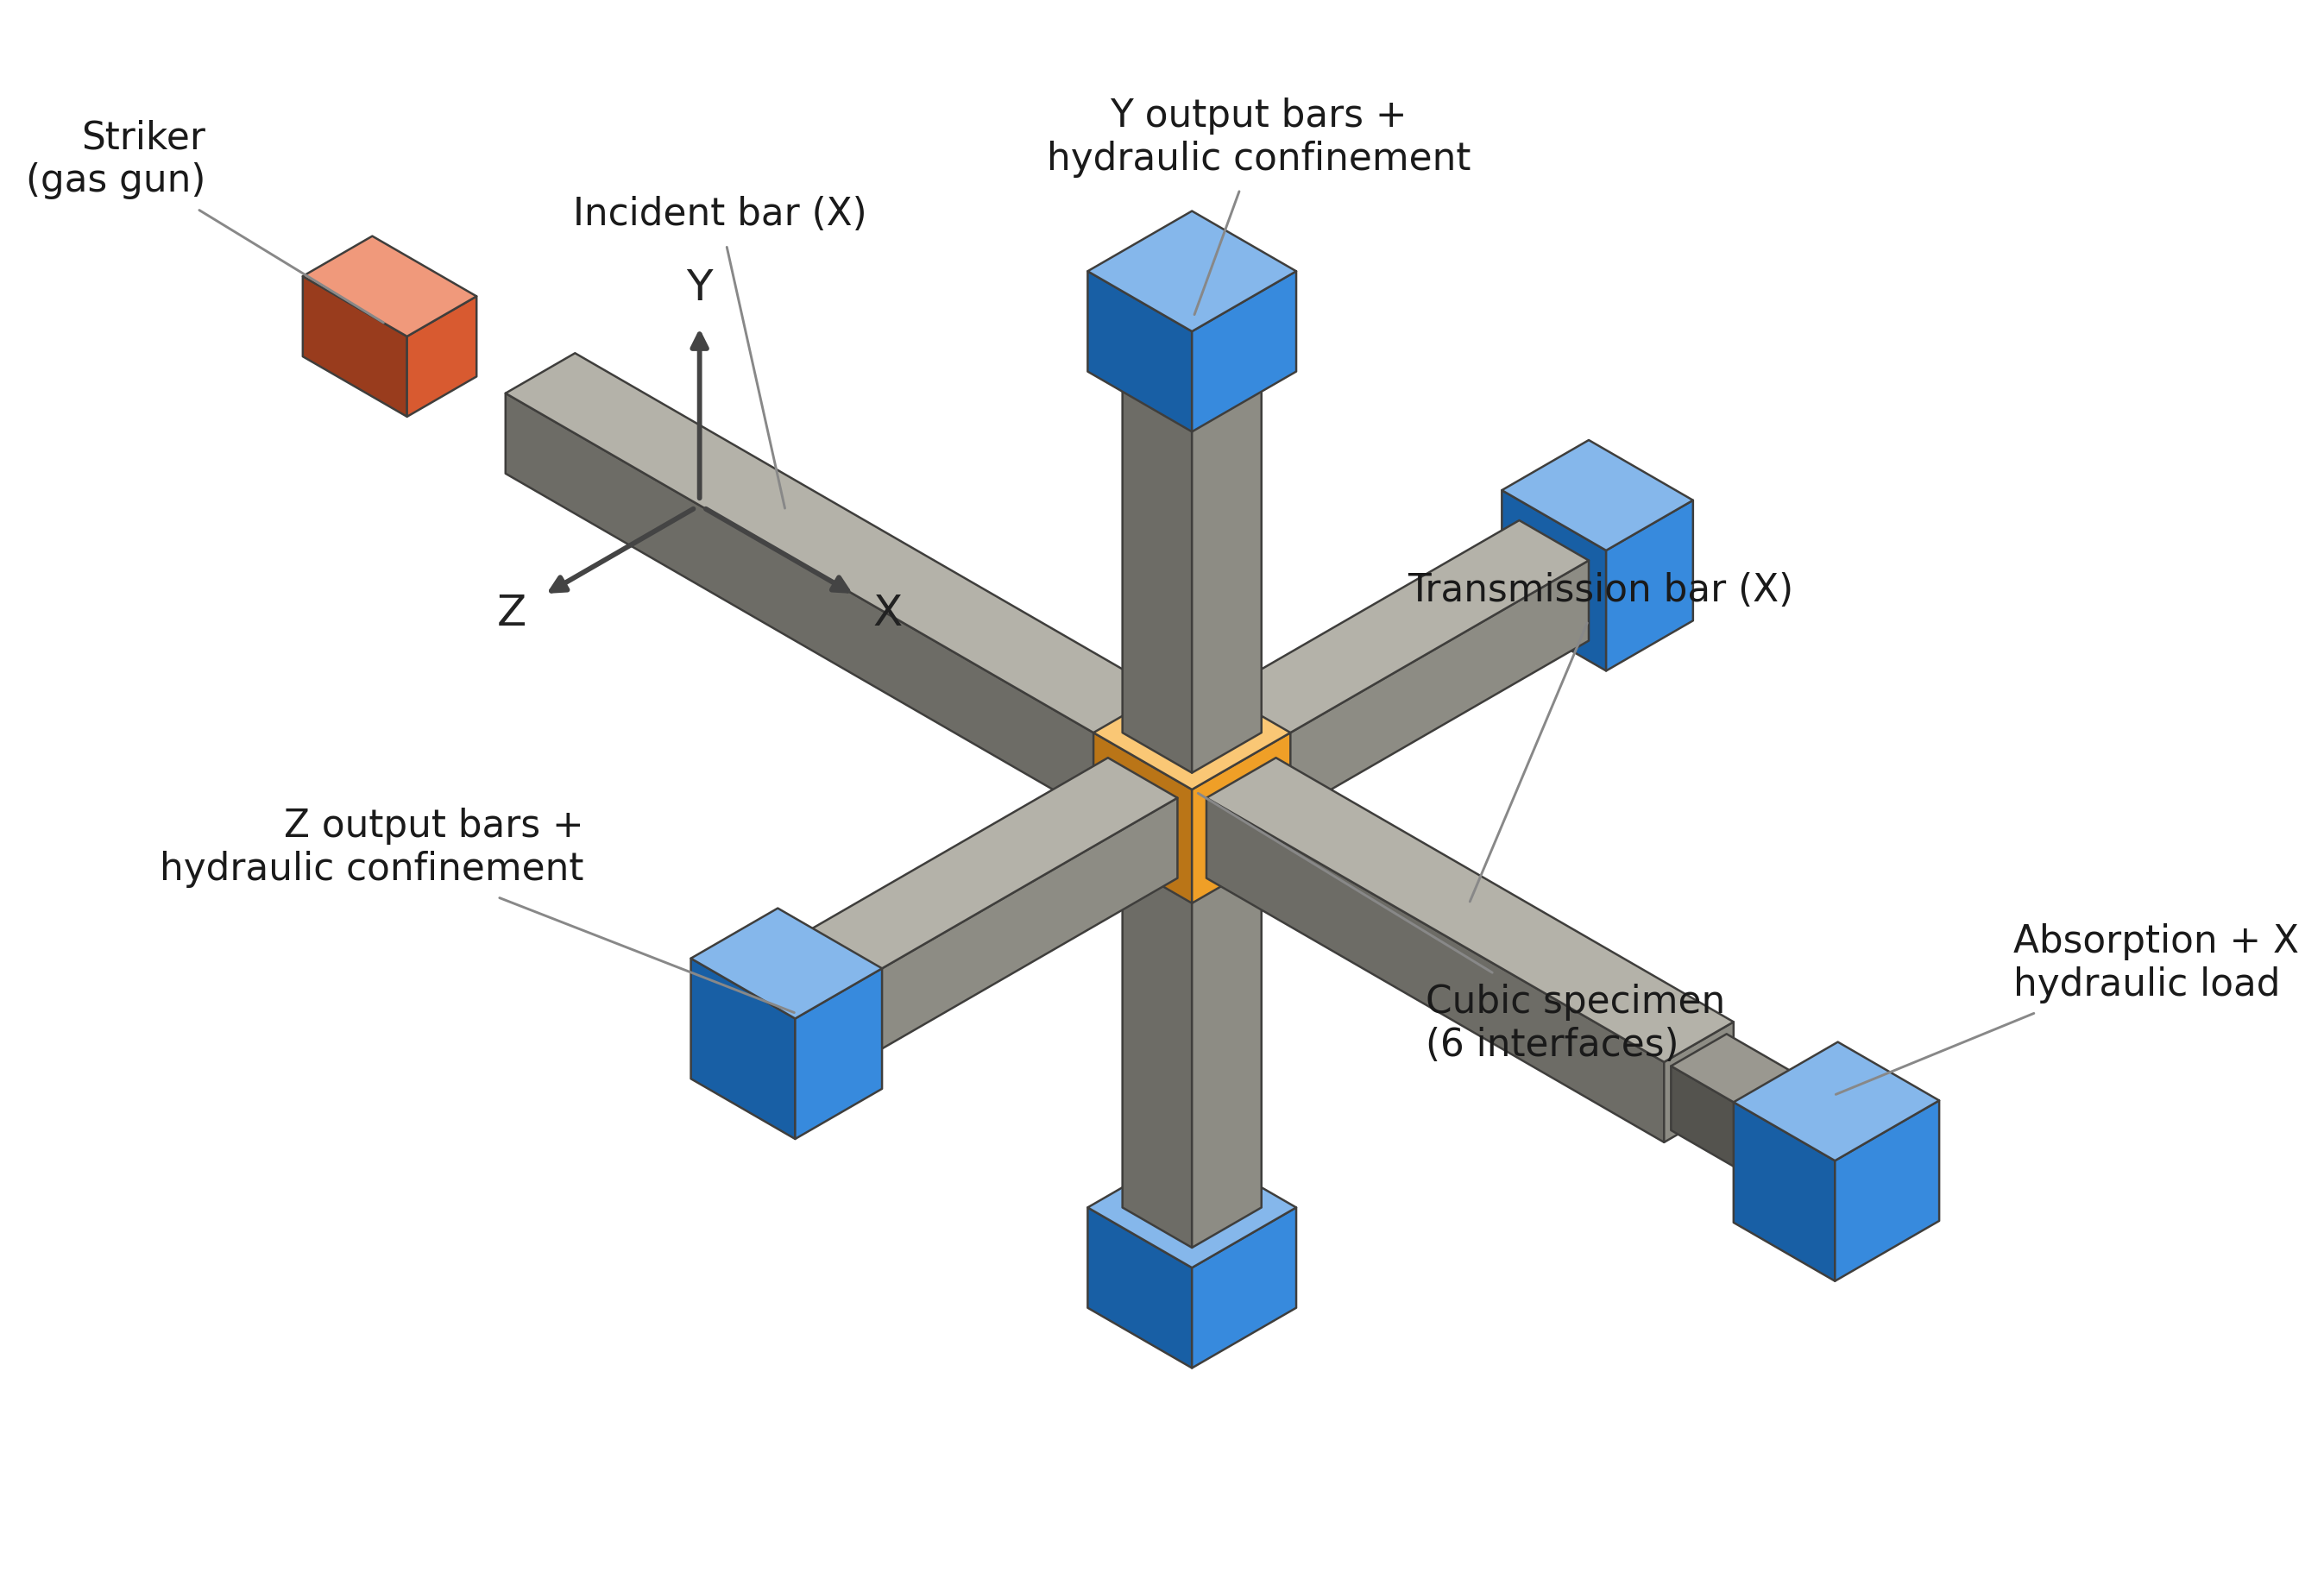
\includegraphics[width=0.92\linewidth]{trihb_system_schematic.png}
  \caption{Isometric schematic of the Monash Tri-HB. The gas gun drives the $X$
  incident/transmission train; two output-bar pairs on $Y$ and $Z$ and a
  hydraulic load cylinder on $X$ apply independent confinement, giving
  static--dynamic coupled true-triaxial loading on the central cubic specimen.}
  \label{fig:schematic}
\end{figure}

\begin{table}[t]
  \centering
  \caption{Representative Monash Tri-HB bar and loading parameters (42CrMo steel).}
  \label{tab:bar}
  \begin{tabular}{lll}
    \toprule
    Quantity & Symbol & Value \\
    \midrule
    Bar density & $\rho_b$ & \SI{7850}{kg/m^3} \\
    Bar Young's modulus & $E_b$ & \SI{210}{GPa} \\
    Bar wave speed & $\Cz$ & \SI{5200}{m/s} \\
    Bar yield strength & $\sigma_y$ & \SI{930}{MPa} \\
    Striker (diameter, length) & $\diameter,\,L_s$ & \SI{40}{mm}, \SI{0.5}{m} \\
    Square-bar cross-section & $A_b$ & \SI{50}{mm}\,$\times$\,\SI{50}{mm} \\
    Incident / transmission / output bar & $L$ & \num{2.5} / \num{2.0} / \SI{2.0}{m} \\
    Maximum impact velocity & $v$ & \SI{50}{m/s} \\
    Hydraulic confinement capacity & $p_c$ & \SI{100}{MPa} \\
    Gauge sampling rate & --- & \SI{1}{MHz} \\
    \bottomrule
  \end{tabular}
\end{table}

\subsection{Four loading families}

The digital twin exposes the system as four top-level loading families, the last
of which branches into three electromagnetic (EM) topologies, giving six physics
modes in total (Table~\ref{tab:families}). This taxonomy spans the historical
uniaxial SHPB (Mode~1), passively or actively confined SHPB (Mode~2), the
gas-gun Tri-HB static--dynamic configuration (Mode~3), and EM programmable
loading (Modes~4--6) in which the pulse on each axis is prescribed independently.
Modes~3 and~5 realise the true-triaxial capability that distinguishes the system.

\begin{table}[t]
  \centering
  \caption{Loading families and the six physics modes of the Virtual Tri-HB.}
  \label{tab:families}
  \small\setlength{\tabcolsep}{4.5pt}
  \begin{tabular}{cllc}
    \toprule
    Mode & Loading family & Topology / variant & True-triaxial \\
    \midrule
    1 & Gas-gun uniaxial SHPB & single $X$ axis & no \\
    2 & Confinement-chamber SHPB & $X$ axis, passive lateral $p_c$ & partial \\
    3 & Gas-gun Tri-HB static--dynamic & $X$ dynamic, $Y,Z$ pre-stress & yes \\
    4 & EM programmable & single-axis one-sided & no \\
    5 & EM programmable & multi-axis one-sided ($X,XY,XYZ$) & yes \\
    6 & EM programmable & symmetric opposing ($\pm X\pm Y\pm Z$) & yes (hydrostatic) \\
    \bottomrule
  \end{tabular}
\end{table}

\begin{figure}[t]
  \centering
  \begin{subfigure}[b]{0.49\linewidth}
    
\includegraphics[width=\linewidth]{mode_1_gas_gun_uniaxial_stress_path.png}
    \caption{Mode 1 --- gas-gun uniaxial SHPB}
  \end{subfigure}\hfill
  \begin{subfigure}[b]{0.49\linewidth}
    
\includegraphics[width=\linewidth]{mode_3_monash_tri_hb_stress_path.png}
    \caption{Mode 3 --- gas-gun Tri-HB}
  \end{subfigure}

  \begin{subfigure}[b]{0.49\linewidth}
    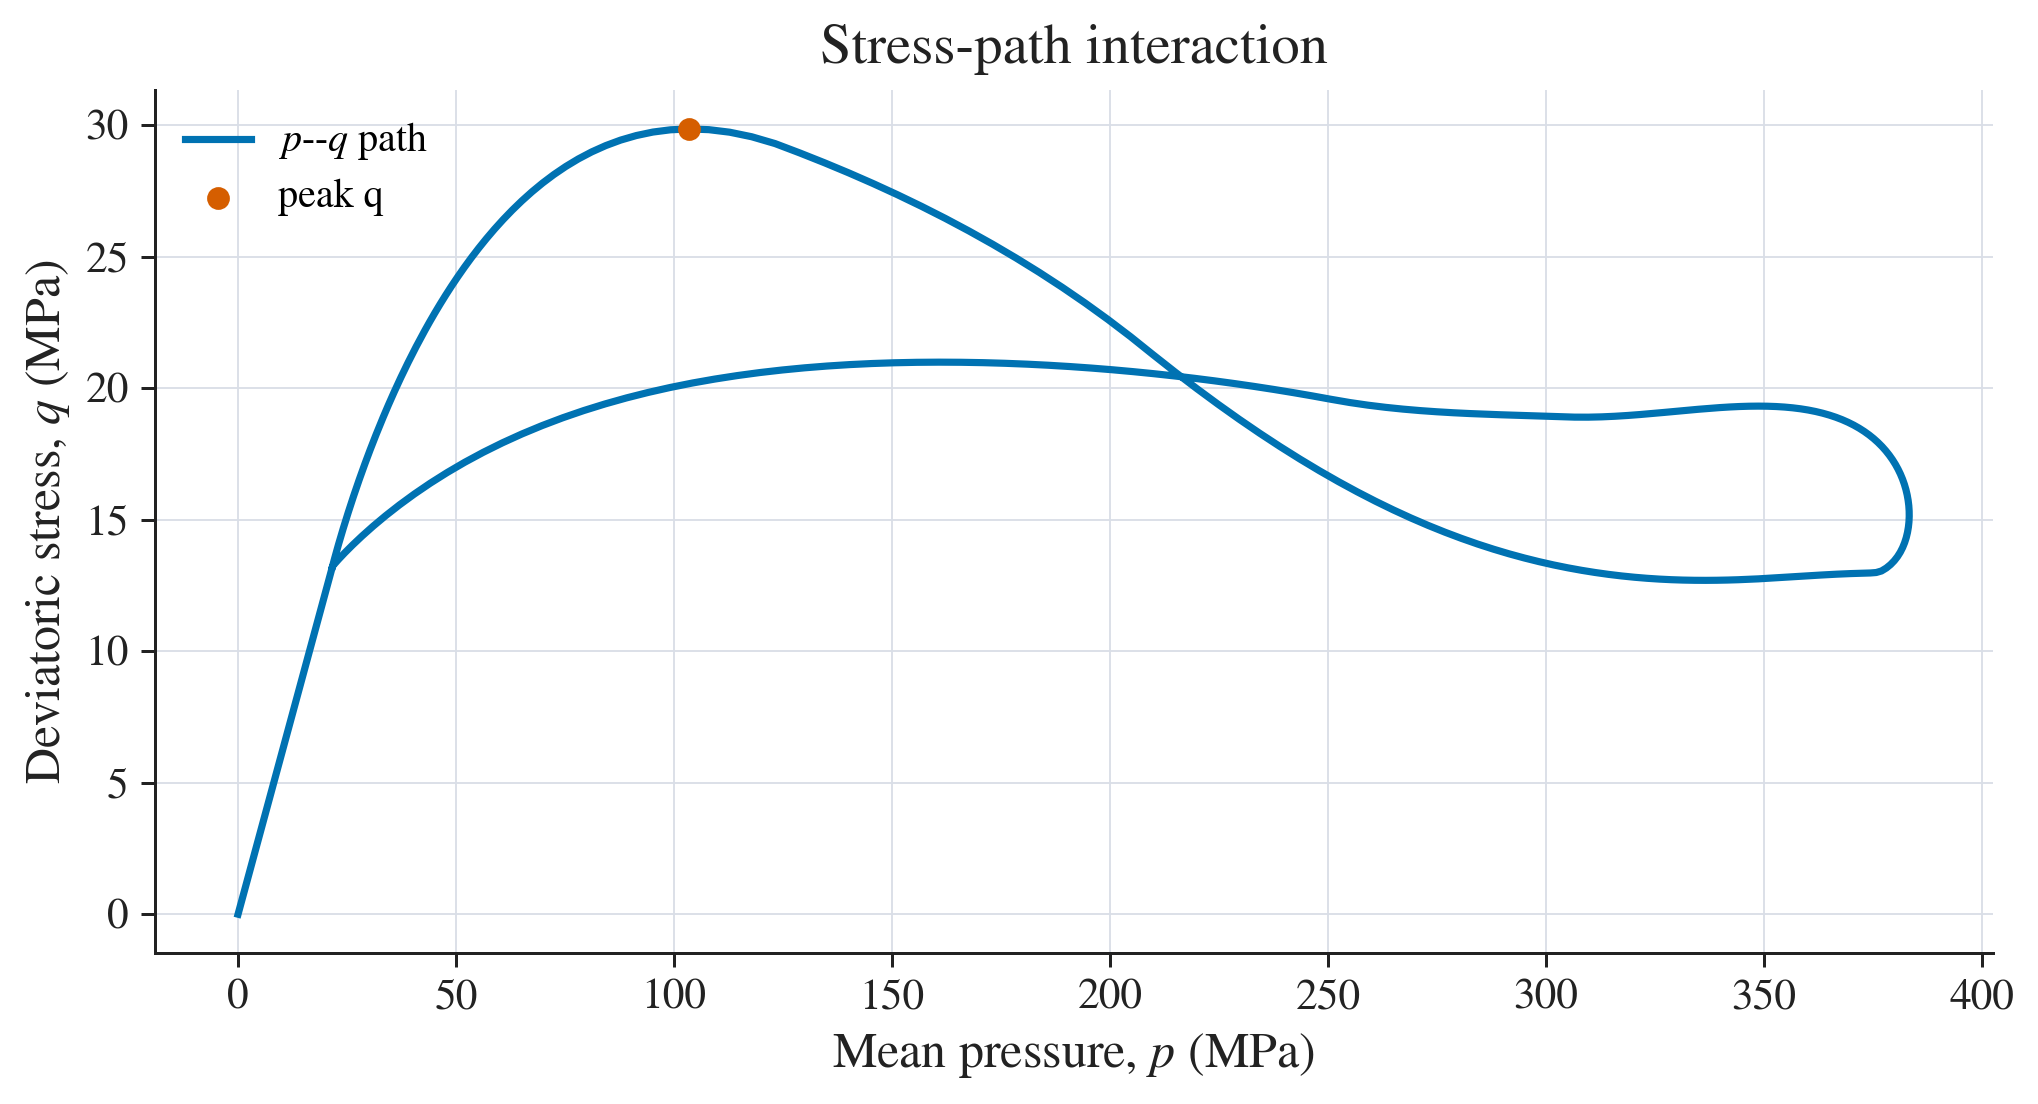
\includegraphics[width=\linewidth]{mode_5_em_async_triaxial_stress_path.png}
    \caption{Mode 5 --- EM asynchronous triaxial}
  \end{subfigure}\hfill
  \begin{subfigure}[b]{0.49\linewidth}
    
\includegraphics[width=\linewidth]{mode_6_em_symmetric_xyz_stress_path.png}
    \caption{Mode 6 --- EM symmetric hydrostatic}
  \end{subfigure}
  \caption{Mean-pressure--deviatoric-stress ($p$--$q$) trajectories for four of
  the six modes. Uniaxial loading (a) traces a steep deviatoric path; the
  triaxial modes (b, c) populate the multiaxial $p$--$q$ plane, and the symmetric
  hydrostatic mode (d) collapses onto the $q\approx0$ axis. The spread of
  accessible stress paths is the analytical advantage of the Tri-HB.}
  \label{fig:modes}
\end{figure}

\section{Per-axis data reduction and wave interaction}\label{sec:reduction}

\subsection{One-dimensional wave propagation and dispersion}\label{sec:wave}

Each pressure bar is a long, slender rod in which, for wavelengths much greater
than the bar diameter, the axial displacement $u(x,t)$ obeys the
one-dimensional elastic wave equation
\begin{equation}
\frac{\partial^2 u}{\partial t^2}=\Cz^2\,\frac{\partial^2 u}{\partial x^2},
\qquad \Cz=\sqrt{E_b/\rho_b},
\label{eq:wave}
\end{equation}
whose general d'Alembert solution $u=f(x-\Cz t)+g(x+\Cz t)$ superposes
forward- and backward-travelling parts. For a wave travelling in a single
direction the axial strain and particle velocity are proportional, giving the
Hopkinson identity
\begin{equation}
v(x,t)=-\Cz\,\eps(x,t),
\label{eq:hopkinson}
\end{equation}
which underlies all bar-gauge analysis: a resistance gauge that measures strain
also measures the particle velocity through the bar wave speed.

At a planar interface between media of acoustic impedance $Z=\rho c$, continuity
of traction and velocity gives the stress reflection and transmission
coefficients\footnote{For a 42CrMo steel bar
$Z_b=\rho_b\Cz\approx4.06\times10^{7}\,\mathrm{kg\,m^{-2}\,s^{-1}}$.}
\begin{equation}
R=\frac{\sigma_R}{\sigma_I}=\frac{Z_2-Z_1}{Z_1+Z_2},\qquad
T=\frac{\sigma_T}{\sigma_I}=\frac{2Z_2}{Z_1+Z_2}.
\label{eq:fresnel}
\end{equation}
For a rock specimen softer than the steel bars ($Z_s<Z_b$) the reflection
coefficient is negative, so the reflected pulse is tensile --- the origin of the
negative reflected strain $\eps_{\mathrm{re}}$ recorded in compression tests, and
a sign-diagnostic of the impedance match.

Equation~\eqref{eq:wave} is exact only in the long-wavelength limit. The exact
axisymmetric (Pochhammer--Chree) solution makes the phase velocity
frequency-dependent, $c_\phi(ka)=\Cz\,\Phi(ka,\nu_b)$, where $k$ is the wavenumber
and $a$ the bar radius: $\Phi\approx1$ for $ka\lesssim0.1$ but falls by a few
percent as $ka\to1$, so an unshaped rectangular pulse --- rich in high-$ka$
harmonics --- develops spurious oscillations as it travels. Dispersion is
negligible while the rise time $\tau_r$ satisfies $a/(c_\phi\tau_r)\lesssim0.1$.
The Tri-HB therefore uses pulse-shaped (gas-gun) and half-sine (electromagnetic)
incident waves, which concentrate their energy at $ka\ll1$ and are essentially
dispersion-free for the bar geometries used here; the digital twin represents
every loading mode with a smooth half-sine incident wave for the same reason.

\subsection{Force--velocity continuity and the three-wave method}

At the incident-bar/specimen face the bar carries the superposed incident and
reflected waves, while the transmission bar carries only the outgoing wave, so the
two face forces and velocities are
\begin{equation}
F_1=E_bA_b\,(\eps_{\mathrm{in}}+\eps_{\mathrm{re}}),\quad
v_1=\Cz(\eps_{\mathrm{in}}-\eps_{\mathrm{re}});\qquad
F_2=E_bA_b\,\eps_{\mathrm{tr}},\quad
v_2=\Cz\,\eps_{\mathrm{tr}}.
\label{eq:faces}
\end{equation}
Once the specimen has reverberated into dynamic stress equilibrium
($t\gtrsim 3\,t_{\mathrm{travel}}$, $t_{\mathrm{travel}}=L_s/c_p$), the average
axial stress, strain rate and strain follow from \eqref{eq:faces} as the standard
three-wave relations
\begin{align}
\sigma_x(t) &= \frac{F_1+F_2}{2A_s}=\frac{E_b A_b}{2 A_s}\big[\eps_{\mathrm{in}}+\eps_{\mathrm{re}}+\eps_{\mathrm{tr}}\big]
            = \frac{E_b A_b}{A_s}\,\eps_{\mathrm{tr}}(t), \\
\epsd(t)    &= \frac{v_1-v_2}{L_s}=\frac{\Cz}{L_s}\big[\eps_{\mathrm{in}}-\eps_{\mathrm{re}}-\eps_{\mathrm{tr}}\big]
            = -\frac{2\Cz}{L_s}\,\eps_{\mathrm{re}}(t), \qquad
\eps(t)=\int_0^t \epsd\,\mathrm{d}\tau,
\end{align}
where $A_b,A_s$ are the bar and specimen cross-sections and $L_s$ the specimen
length; the right-hand (one-wave) forms hold under perfect equilibrium
$\eps_{\mathrm{in}}+\eps_{\mathrm{re}}=\eps_{\mathrm{tr}}$, and their agreement with the
two-face forms is the reducer's built-in equilibrium check. Equilibrium itself is
quantified by the force-balance ratio
\begin{equation}
\mathcal{R}(t)=\frac{|F_1(t)-F_2(t)|}{\tfrac12\big(F_1(t)+F_2(t)\big)}<0.05,
\qquad t_{\mathrm{eq}}\approx(3\text{--}5)\,L_s/c_p.
\label{eq:equil}
\end{equation}
The lateral response is obtained from the two output bars on each transverse axis,
\begin{equation}
\sigma_y(t)=\frac{E_b A_b}{2A_s}\big[\eps_{y1}+\eps_{y2}\big],\qquad
\sigma_z(t)=\frac{E_b A_b}{2A_s}\big[\eps_{z1}+\eps_{z2}\big],
\end{equation}
with the analogous strain integrals. These lateral outputs are Poisson-driven:
the $X$ pulse compresses the specimen, which expands laterally and drives output
waves outward along the $Y$ and $Z$ bars, recorded by gauges G3--G6. The Virtual
Tri-HB performs this reduction simultaneously on all three axes, so a single test
yields the full $\sigma_x,\sigma_y,\sigma_z$ history rather than one axial curve.

\subsection{Validity of the three-wave method under static pre-stress}\label{sec:prestress}

In the static--dynamic configuration the hydraulic cylinders pre-load the bars
before the pulse arrives, so the bar ends are no longer free. Because the bar is
linear-elastic, the total field superposes a uniform static part and the
propagating dynamic part, $\sigma=\sigma_s+\sigma_d$ with
$\sigma_s=F_{\mathrm{pre}}/A_b=\mathrm{const}$ ($\mathrm{d}\sigma_s/\mathrm{d}x=0$).
Substituting into \eqref{eq:wave}, the static part drops out and the dynamic part
obeys the same wave equation, so the three-wave relations apply unchanged to the
dynamic \emph{increments} $\eps_{\mathrm{in}},\eps_{\mathrm{re}},\eps_{\mathrm{tr}}$
--- the pre-stress is merely a constant gauge offset, removed by baselining before
the pulse. The superposition is valid provided the bar stays elastic at all times,
\begin{equation}
\sigma_{d,\mathrm{peak}}<\sigma_{\mathrm{prop}}-|\sigma_s|,
\label{eq:budget}
\end{equation}
so the pre-stress consumes part of the dynamic-amplitude budget (the bar-plasticity
limit the workspace enforces); the wave speed $C_0=\sqrt{E_b/\rho_b}$ is unchanged
to within a sub-percent acoustoelastic shift, and the quasi-static actuator leaves
the end's \emph{dynamic} impedance --- and hence the reflection seen by the pulse
--- effectively that of a free bar over the $\mu$s event. This superposition is
what legitimises static--dynamic coupled testing.

\subsection{Wave-interaction regime map}

For multi-axis loading the relative timing of the per-axis pulses controls
whether the specimen responds by wave superposition or by sequential
damage-memory. Defining a normalised inter-axis delay $\Delta t^\ast =
\Delta t / t_{\mathrm{travel}}$, with $t_{\mathrm{travel}}=L_s/c_p$ the
specimen transit time, the workflow classifies the response into synchronous
superposition ($\Delta t^\ast\!<\!1$), reverberation-coupled
($1\!\le\!\Delta t^\ast\!\le\!3$), transitional ($3\!<\!\Delta t^\ast\!\le\!10$)
and sequential damage-memory ($\Delta t^\ast\!>\!10$) regimes
(Fig.~\ref{fig:regime}). This map links the \emph{timing} of triaxial loading to
the \emph{mechanism} of failure, a relationship unique to programmable multiaxial
systems.

\begin{figure}[t]
  \centering
  \begin{subfigure}[b]{0.49\linewidth}
    
\includegraphics[width=\linewidth]{step2_input_dynamic_pulses.png}
    \caption{Per-axis pulse timing}
  \end{subfigure}\hfill
  \begin{subfigure}[b]{0.49\linewidth}
    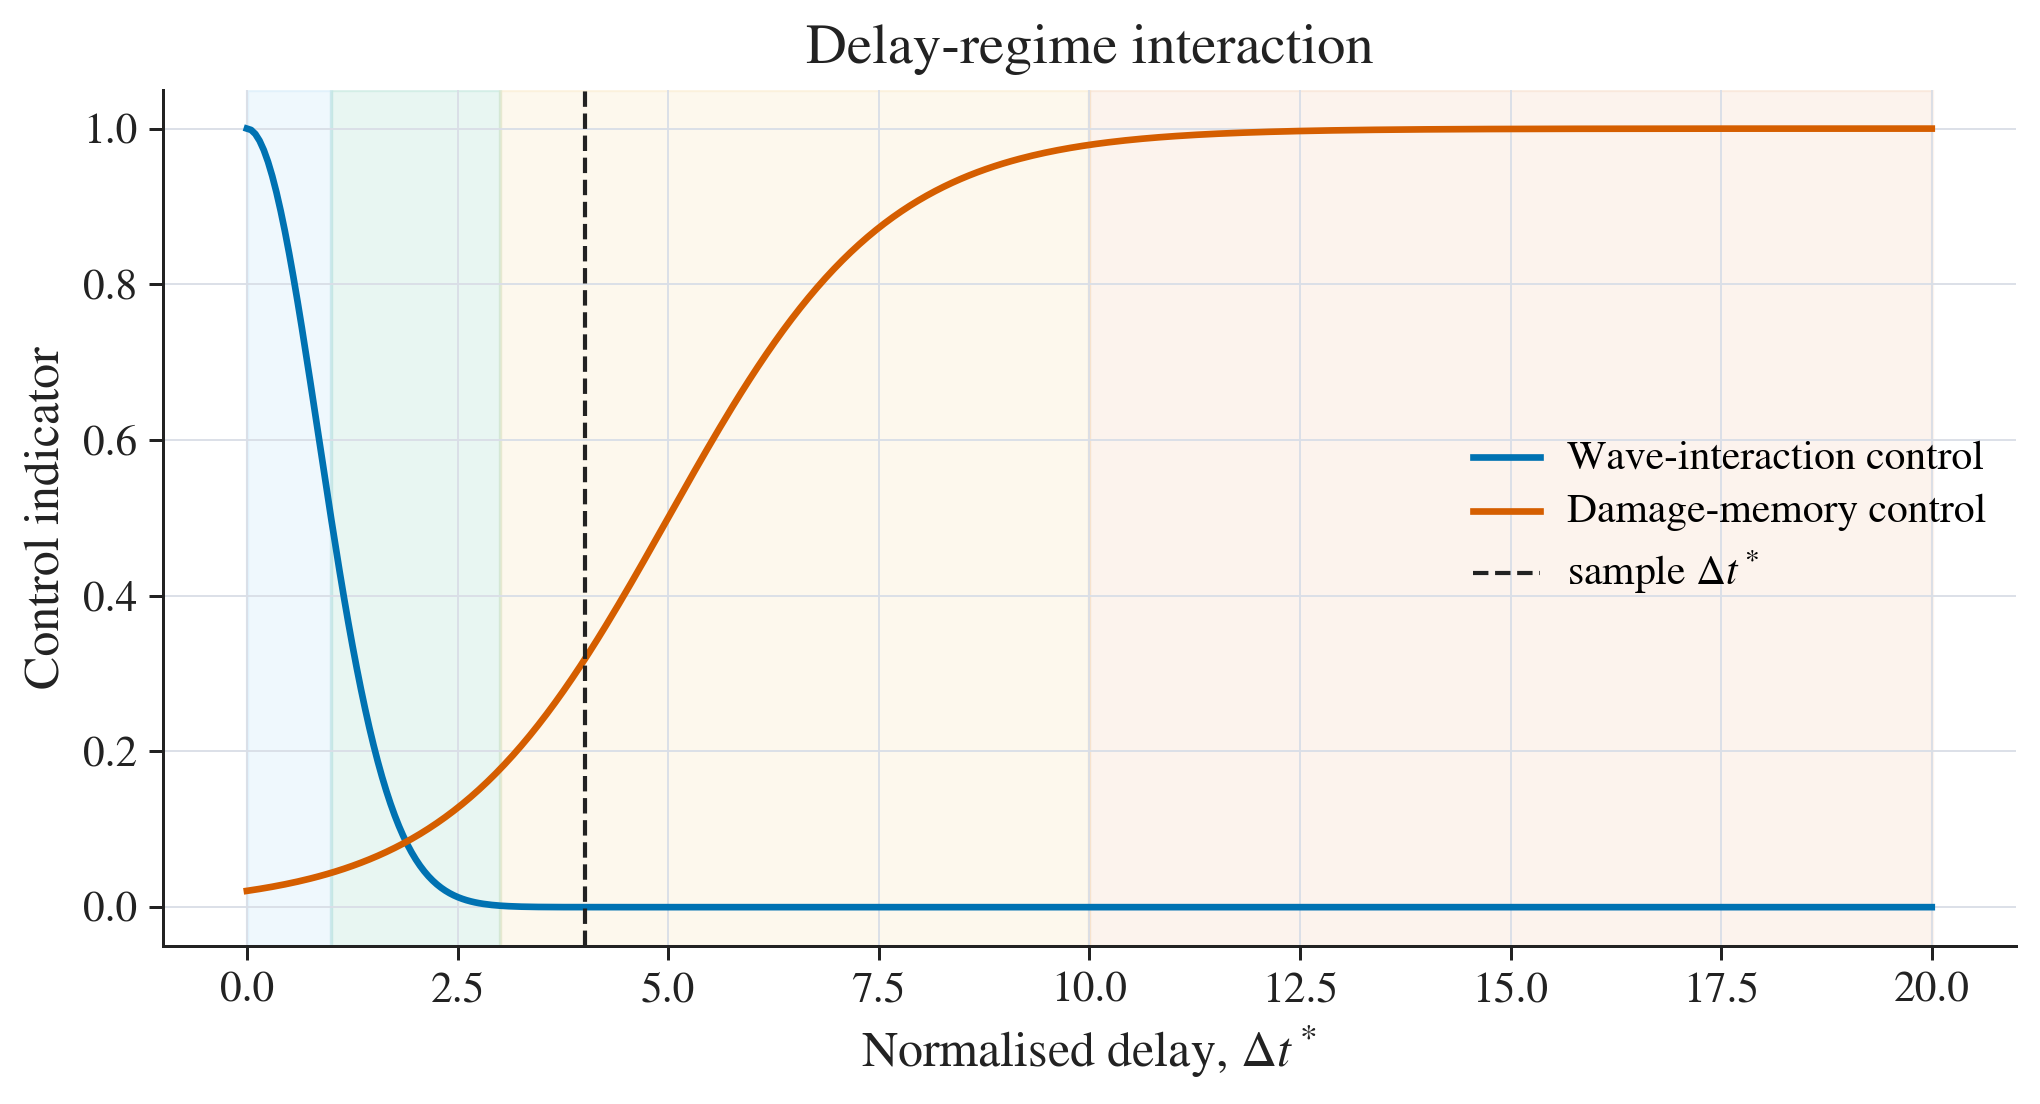
\includegraphics[width=\linewidth]{step2_delay_regime_map.png}
    \caption{Delay-regime interaction map}
  \end{subfigure}
  \caption{Wave-interaction analysis (Step~2). (a) Independently delayed $X$, $Y$,
  $Z$ pulses with the $3$--$5$ travel-time equilibrium window shaded. (b) The
  normalised-delay regime map separating superposition-controlled from
  damage-memory-controlled response.}
  \label{fig:regime}
\end{figure}

\section{The integrated digital twin}\label{sec:twin}

The Virtual Tri-HB (\texttt{tri\_hb\_integrated.py}) is a single application that
bundles six analysis steps under one shared experimental setup: (1) configuration
and either simulation or reduction of bar-gauge data; (2) wave-propagation and
equilibrium analysis; (3) stress-path and invariant analysis; (4) damage and
energy analysis with directional descriptors; (5) a publication-ready summary;
and (6) automatic generation of a report and presentation (\LaTeX{} + PDF) from
the current run. A separate page renders the live calibration/validation plan.
Each step inherits the shared configuration, so the wave, stress-path and damage
views remain mutually consistent. The stress-path stage resolves the total
stresses into the invariants
\begin{equation}
p=\tfrac{1}{3}(\sigma_x+\sigma_y+\sigma_z),\quad
q=\sqrt{\tfrac{1}{2}\big[(\sigma_x-\sigma_y)^2+(\sigma_y-\sigma_z)^2+(\sigma_z-\sigma_x)^2\big]},\quad
\cos 3\theta=\frac{3\sqrt3}{2}\frac{J_3}{J_2^{3/2}},
\end{equation}
so that all three principal stresses --- including the intermediate stress
through the Lode angle $\theta$ --- enter the subsequent failure analysis
(Fig.~\ref{fig:stresspath}).

\begin{figure}[t]
  \centering
  \begin{subfigure}[b]{0.49\linewidth}
    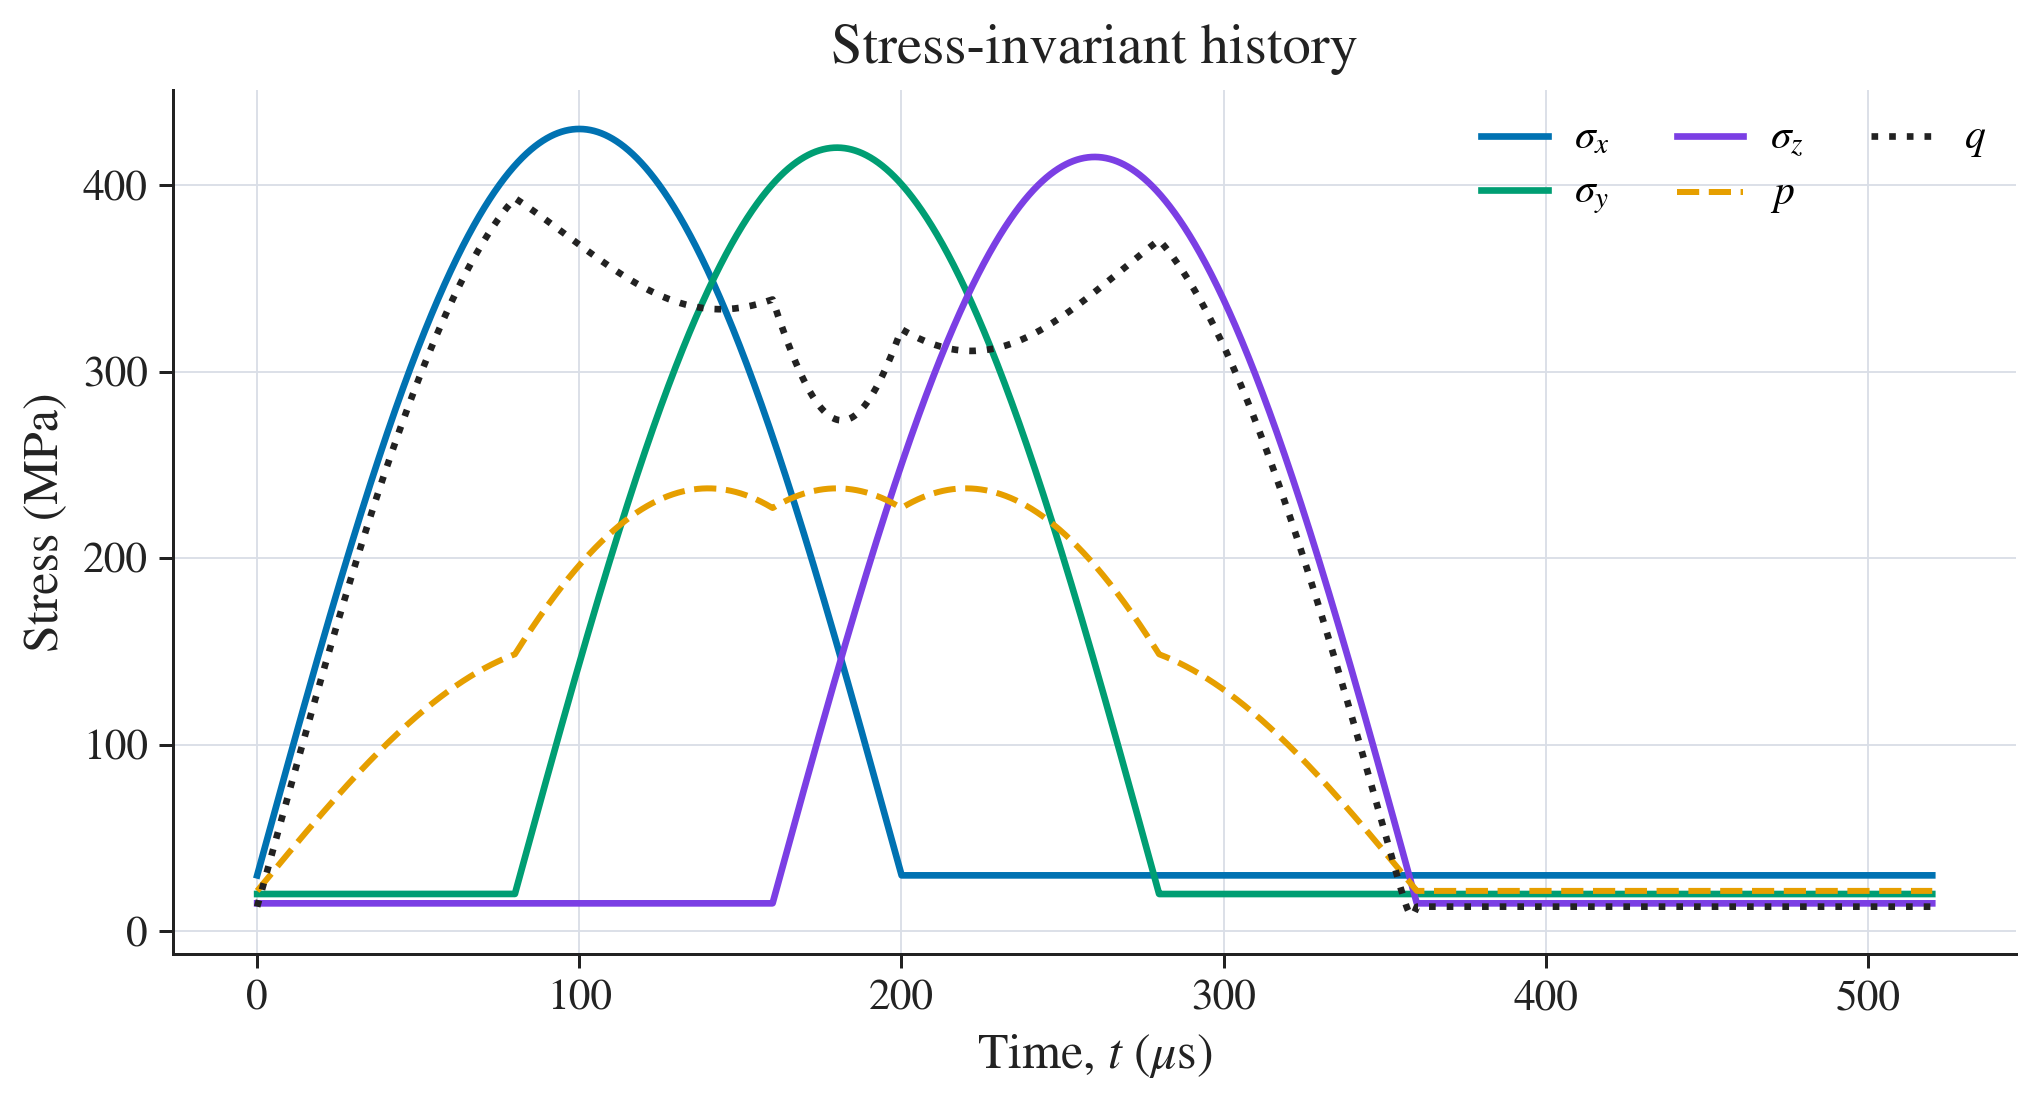
\includegraphics[width=\linewidth]{step3_total_stresses_invariants.png}
    \caption{Stress and invariant histories}
  \end{subfigure}\hfill
  \begin{subfigure}[b]{0.49\linewidth}
    
\includegraphics[width=\linewidth]{step3_pq_trajectory.png}
    \caption{$p$--$q$ trajectory (time-coloured)}
  \end{subfigure}
  \caption{Stress-path analysis (Step~3) for the reference asynchronous-XYZ case:
  total principal stresses with the mean and deviatoric invariants (a), and the
  resulting $p$--$q$ trajectory traced in time (b).}
  \label{fig:stresspath}
\end{figure}

\section{Constitutive advances}\label{sec:advances}

\subsection{True-triaxial, rate-dependent failure envelope}\label{sec:env}

Failure is evaluated through the index $F=q/q_f$ against a pressure-dependent
envelope with a deviatoric (Lode) shape and an optional rate dependence,
\begin{equation}
q_f=(A_{\mathrm{eff}}+B_{\mathrm{eff}}\,p^{\,n})\,h(\theta),\qquad
A_{\mathrm{eff}}=A\,\mathrm{DIF},\quad
\mathrm{DIF}=1+b_{\mathrm{env}}\log_{10}\!\max\!\Big(\tfrac{|\epsd_{\mathrm{eq}}|}{\epsd_0},1\Big).
\label{eq:qf}
\end{equation}
The meridian intercept and slope $A,B$ are derived consistently from the
unconfined strength and confinement ratio, ensuring $F=1$ at the static failure
point. The deviatoric shape $h(\theta)$ admits three forms: a legacy cap, a
linear extension-weakened interpolation, and a convex Willam--Warnke
form~\citep{willam1975}. Both new forms use the meridian ratio $\rho_t/\rho_c$
and make the extension meridian \emph{weaker} than compression --- the physically
correct sense for brittle rock --- so the intermediate principal stress effect
enters with the right sign (Fig.~\ref{fig:envelope}a). The default is the Lode
form with $\rho_t/\rho_c=0.70$. The optional rate term in Eq.~\eqref{eq:qf}
inflates the envelope with strain rate (Fig.~\ref{fig:envelope}b), so that the
\emph{onset} of failure shifts dynamically, complementing the rate sensitivity of
the damage kinetics~\citep{zhao2000}.

\begin{figure}[t]
  \centering
  \begin{subfigure}[b]{0.49\linewidth}
    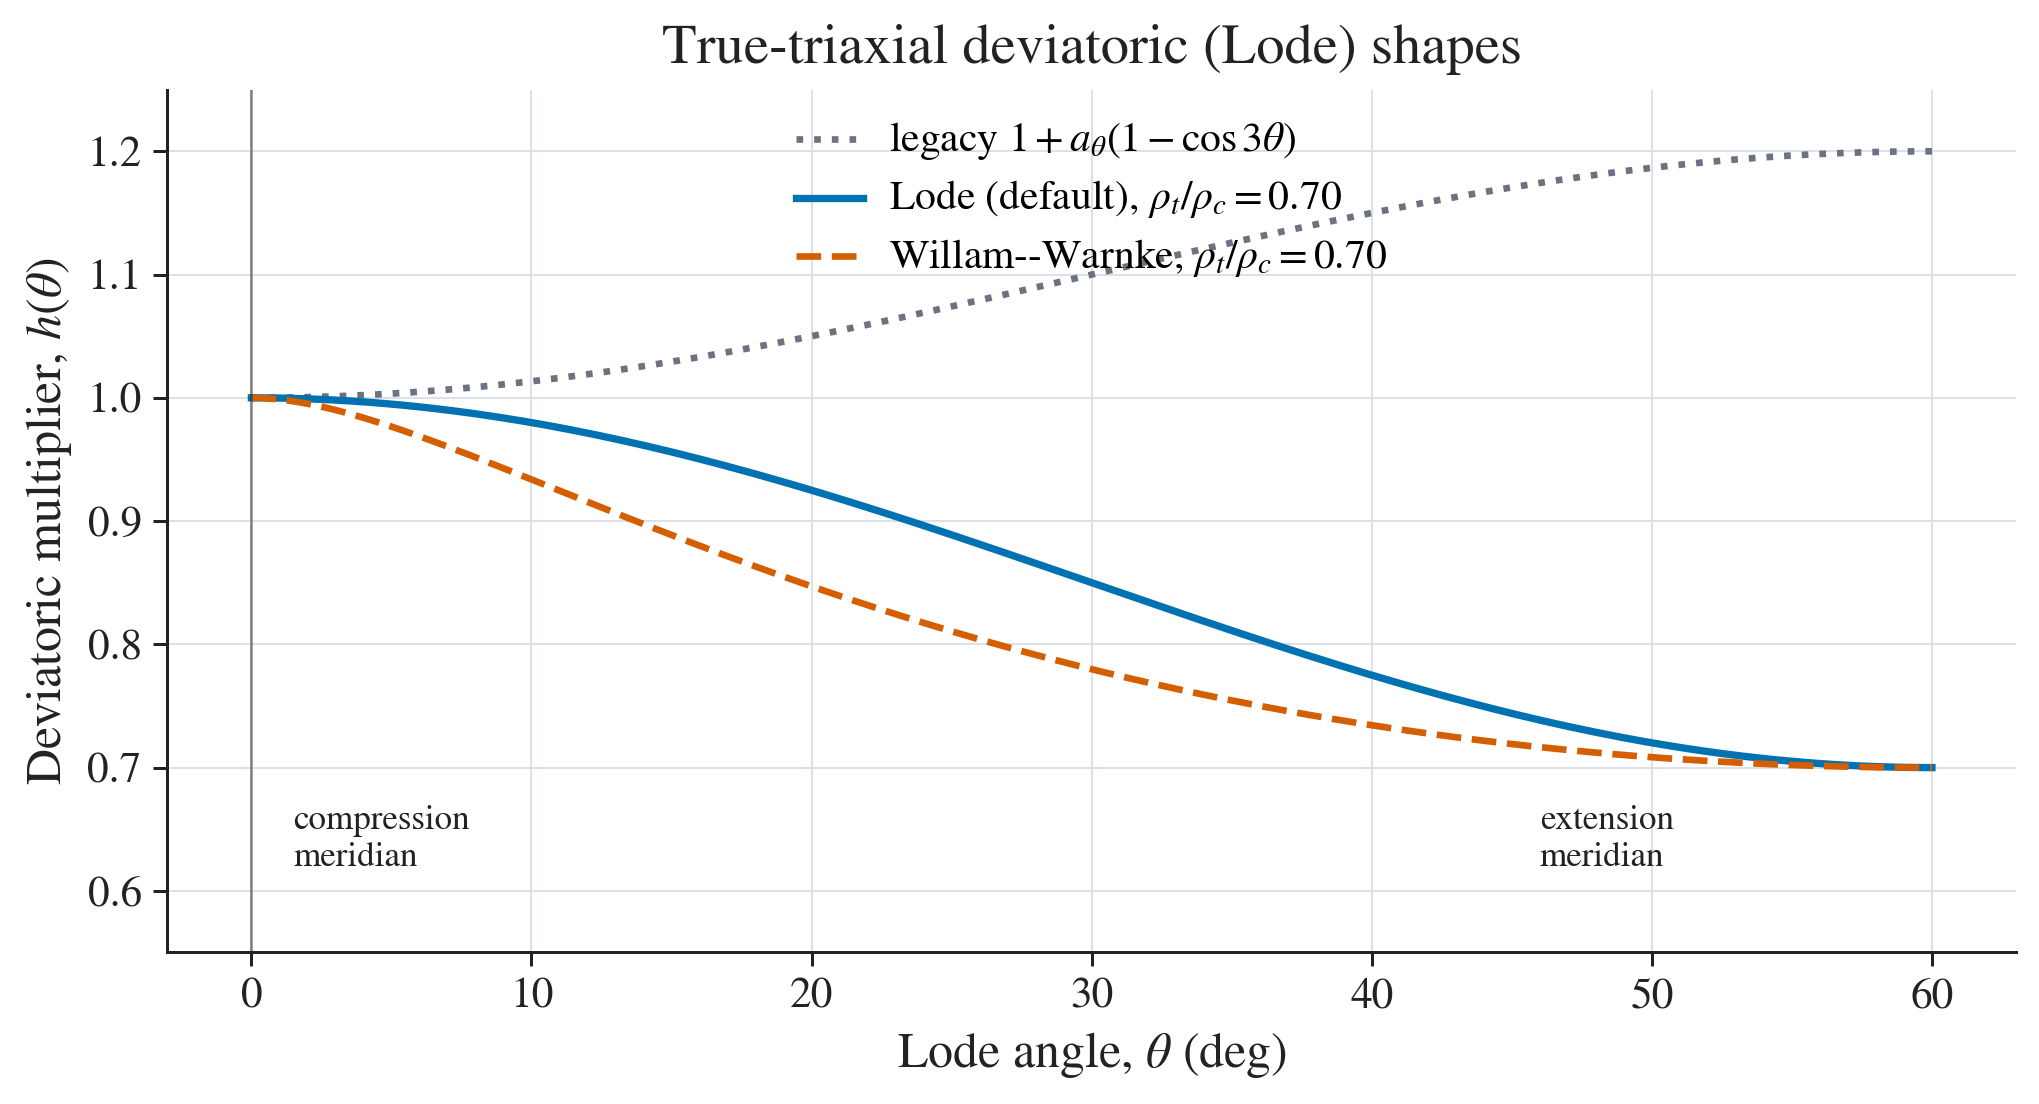
\includegraphics[width=\linewidth]{step3_lode_shapes.png}
    \caption{Deviatoric (Lode) shapes}
  \end{subfigure}\hfill
  \begin{subfigure}[b]{0.49\linewidth}
    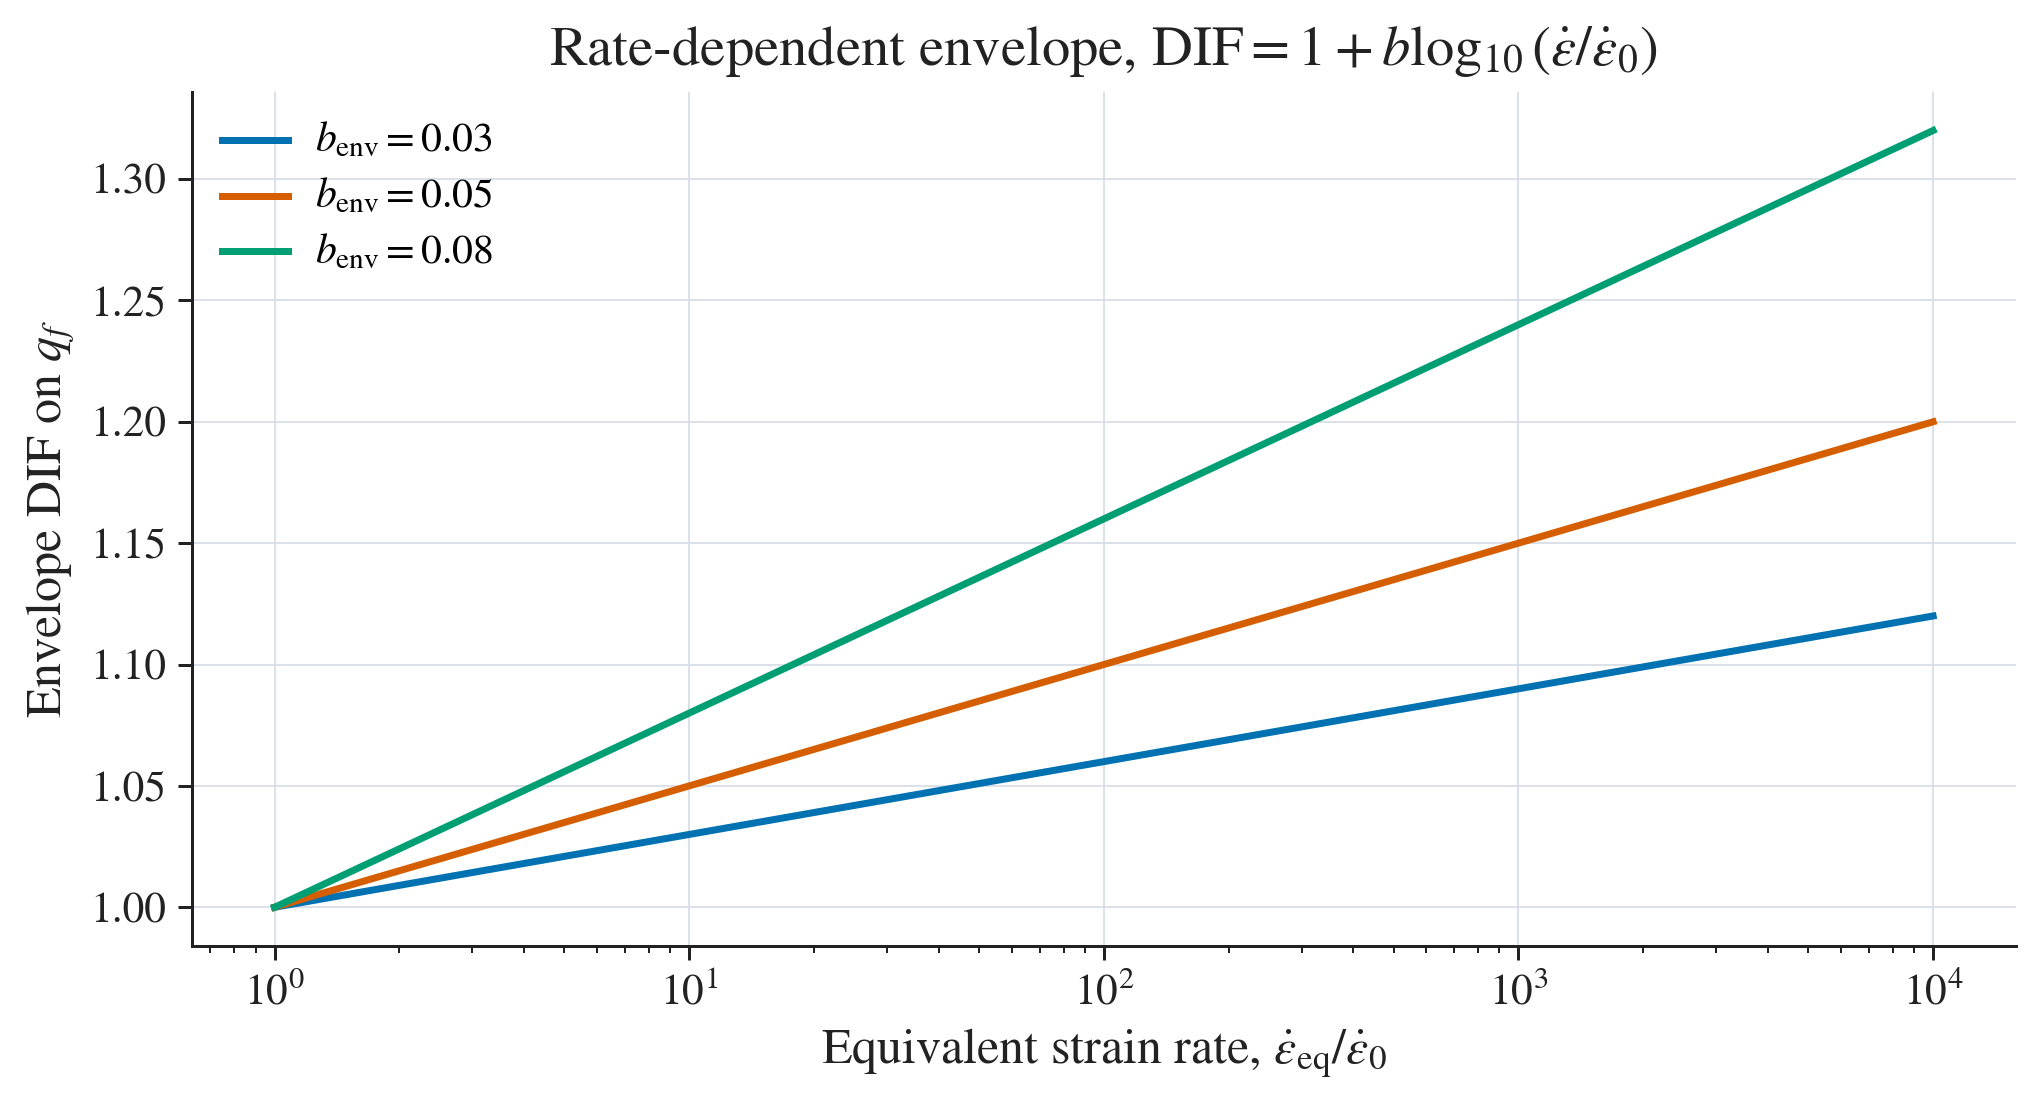
\includegraphics[width=\linewidth]{step3_rate_dependent_envelope.png}
    \caption{Envelope dynamic increase factor}
  \end{subfigure}
  \caption{True-triaxial and rate-dependent failure envelope. (a) The default
  Lode and Willam--Warnke shapes correctly weaken the extension meridian relative
  to compression ($\rho_t/\rho_c=0.70$), capturing the $\sigma_2$ effect; the
  legacy cap (dotted) has the opposite, unphysical sense. (b) Optional envelope
  DIF versus normalised strain rate.}
  \label{fig:envelope}
\end{figure}

\subsection{Thermodynamically consistent damage dissipation}\label{sec:energy}

Damage $D$ evolves by a Perzyna-type overstress law with load-shedding feedback,
\begin{equation}
\dot D=\frac{(1-D)^{\alpha}}{\tau_D}
\Big\langle\frac{F_{\mathrm{eff}}-1}{F_0}\Big\rangle^{m}
\Big(\frac{|\epsd_{\mathrm{eq}}|}{\epsd_0}\Big)^{\beta},
\qquad F_{\mathrm{eff}}=(1-D)\,F,
\label{eq:damage}
\end{equation}
so that $D$ self-limits rather than snapping to unity~\citep{perzyna1966,lemaitre1985}.
Crucially, the energy partition is now derived from a single constitutive
relation. Damage degrades the secant modulus to $E_0(1-D)$, so the specimen
carries the damage-coupled elastic strain and the work, recoverable energy and
dissipation become
\begin{equation}
\varepsilon_i=\frac{\sigma_i-\nu(\sigma_j+\sigma_k)}{E_0(1-D)},\quad
W_{\mathrm{input}}=\!\int_0^t\!\sigma_i\dot\varepsilon_i\,\mathrm{d}\tau,\quad
W_{\mathrm{el}}=\tfrac12\sigma_i\varepsilon_i,\quad
W_{\mathrm{diss}}=W_{\mathrm{input}}-W_{\mathrm{el}}\ge 0 .
\end{equation}
The first law then closes by construction,
$W_{\mathrm{input}}=W_{\mathrm{el}}+W_{\mathrm{diss}}$: the input work ends above
zero by exactly the dissipated part, the recoverable energy returns toward zero on
unloading, and the dissipation rises monotonically (Fig.~\ref{fig:energy}). This
removes the inconsistency of treating the input work as fully recoverable while
estimating dissipation from a separate integral.

\begin{figure}[t]
  \centering
  
\includegraphics[width=0.62\linewidth]{step4_energy_density_histories.png}
  \caption{Energy-density partition (Step~4). With the damage-coupled strain the
  balance closes exactly: $W_{\mathrm{input}}=W_{\mathrm{el}}+W_{\mathrm{diss}}$,
  with $W_{\mathrm{diss}}$ the non-recoverable (dissipated) energy.}
  \label{fig:energy}
\end{figure}

\subsection{Orthotropic damage for blasting-induced fracturing}\label{sec:ortho}

Rock blasting produces \emph{directional} fracture: radial cracks and spall open
perpendicular to the local tension, so the stiffness and wave-speed loss differ
by direction. A scalar $D$ cannot represent this. The Tri-HB digital twin
therefore offers a diagonal damage tensor $\mathbf{D}=\mathrm{diag}(D_x,D_y,D_z)$
aligned with the bars, each component driven by the directional tensile
(extensile) strain through the same overstress kinetics,
\begin{equation}
\dot D_i=\frac{(1-D_i)^{\alpha}}{\tau_D}
\Big\langle\frac{(1-D_i)F_i-1}{F_0}\Big\rangle^{m}
\Big(\frac{|\epsd_{\mathrm{eq}}|}{\epsd_0}\Big)^{\beta},\qquad
F_i=\frac{\langle-\varepsilon_i\rangle_+}{\varepsilon_{t0}},\quad
\varepsilon_{t0}=\frac{\sigma_t}{E_0},
\end{equation}
for $i=x,y,z$. Damage grows only under directional extension --- there is no
damage in pure compression --- so axial $X$ compression drives the lateral
components $D_y,D_z$ (axial splitting) while $D_x\!\approx\!0$, and confinement on
an axis suppresses its damage (Fig.~\ref{fig:ortho}a). The per-axis modulus
degrades independently, $E_i=E_0(1-D_i)$ (Fig.~\ref{fig:ortho}b), as does the
directional wave speed $c_{p,i}=c_{p0}\sqrt{1-D_i}$. This formulation is rooted
in the microcrack-damage tradition for brittle rock~\citep{grady1980,taylor1986}
but resolves damage by direction. Decisively, because the three orthogonal bars
measure direction-resolved modulus and wave-speed loss, each $D_i$ can be
calibrated \emph{component-by-component} from a single true-triaxial test --- a
measurement a uniaxial SHPB cannot provide.

\begin{figure}[t]
  \centering
  \begin{subfigure}[b]{0.49\linewidth}
    
\includegraphics[width=\linewidth]{step4_orthotropic_damage.png}
    \caption{Damage-tensor components $D_x,D_y,D_z$}
  \end{subfigure}\hfill
  \begin{subfigure}[b]{0.49\linewidth}
    
\includegraphics[width=\linewidth]{step4_directional_stiffness.png}
    \caption{Directional stiffness $E_i=E_0(1-D_i)$}
  \end{subfigure}
  \caption{Orthotropic (Stage-1) damage for the reference triaxial case. (a) The
  diagonal damage-tensor components, each grown by its own directional tensile
  strain; the scalar $D=\max_i D_i$ governs the energy/stiffness summary. (b) The
  resulting directional modulus loss, the per-axis quantity the three bar pairs
  measure.}
  \label{fig:ortho}
\end{figure}

\section{Validation and calibration roadmap}\label{sec:roadmap}

The advances above are constitutive and computational; the system is presented
here as a measurement-and-modelling framework rather than a validated predictive
model. The decisive step is experimental: a staged, hierarchical calibration
that fixes the elastic and strength parameters before the damage kinetics, on a
\emph{calibration set} of tests, followed by \emph{blind prediction} on a disjoint
\emph{validation set}. The Tri-HB's unique strength is that its three independent
axes allow each anisotropic-damage component, each meridian of the failure
surface and each rate level to be probed directly. A practical matrix calibrates
the meridian and Lode parameters on Modes~1--3 and blind-predicts the EM
multiaxial Modes~4--5, while the directional damage components $D_x,D_y,D_z$ are
recovered post-test from per-axis ultrasonic modulus loss,
$D_i=1-E_{i,\mathrm{post}}/E_0$. Demonstrating that one calibrated parameter set
predicts strength and directional fracture on a held-out loading path is what
converts the framework from phenomenological to predictive, and is the natural
subject of the experimental campaign now enabled by the system.

\section{Conclusions}\label{sec:conclusion}

We have presented the Monash true-triaxial Hopkinson bar and its integrated
digital twin. The principal advances are: (i) a unified four-family, six-mode
treatment that spans uniaxial SHPB to programmable multiaxial loading on a single
shared setup; (ii) a true-triaxial, Lode-angle- and rate-dependent failure
envelope that captures the intermediate principal stress effect with the correct
sign; (iii) a thermodynamically consistent damage-energy partition in which the
first law closes by construction; and (iv) an orthotropic damage tensor whose
directional components reproduce the oriented fracture of rock blasting and can be
calibrated component-by-component from the system's direction-resolved
measurements. Together, the hardware and its digital twin establish a platform
for quantitative, multiaxial dynamic constitutive modelling of rock; the
immediate next step is the experimental calibrate-then-blind-predict campaign
that the system uniquely enables.

\section*{Declarations}

\noindent\textbf{Funding.} Not declared (development study).\\[2pt]
\textbf{Competing interests.} The author declares no competing interests.\\[2pt]
\textbf{Data and code availability.} The Virtual Tri-HB workspace
(\texttt{tri\_hb\_integrated.py}) and the figure-generation scripts used here are
part of the Tri-HB repository. All figures in this paper are produced from
prescribed-pulse reference cases by the workspace's own analysis pipeline; no
experimental data were used.\\[2pt]
\textbf{Author contributions.} Q.B.Z. conceived the system and the digital-twin
framework, implemented the analysis pipeline, and wrote the manuscript.

\printbibliography

\end{document}
